\documentclass[a4paper, 12pt]{article}

%%% SST LAB PROTOCOLL PREAMBLE
%%% 2019
%%%%%%%%%%%%%%%%%%%%%%%%%%%%%%%


%%% PACKAGES
%%%%%%%%%%%%%%%%%%%%%%%%%%%

\usepackage[ngerman]{babel}

\usepackage[utf8]{inputenc}
\usepackage{amsmath}
\usepackage{pgfplots}
\usepackage{tikz}
\usepackage[many]{tcolorbox}
\usepackage{graphicx}
\graphicspath{ {./graphics/} }
\usepackage{pdfpages}
\usepackage{dashrule}
\usepackage{float}
\usepackage{siunitx}
\usepackage{trfsigns}
\usepackage{booktabs}
\usepackage[european]{circuitikz}
\usepackage{tcolorbox}

%%% DOCUMENT GEOMETRY
%%%%%%%%%%%%%%%%%%%%%%%%%%%

\usepackage{geometry}
\geometry{
 a4paper,
 total={0.6180339887498948\paperwidth,0.6180339887498948\paperheight},
 top = 0.1458980337503154\paperheight,
 bottom = 0.1458980337503154\paperheight
 }
\setlength{\jot}{0.013155617496424828\paperheight}
\linespread{1.1458980337503154}

\setlength{\parskip}{0.013155617496424828\paperheight} % paragraph spacing


%%% COLORS
%%%%%%%%%%%%%%%%%%%%%%%%%%%

\definecolor{red1}{HTML}{f38181}
\definecolor{yellow1}{HTML}{fce38a}
\definecolor{green1}{HTML}{95e1d3}
\definecolor{blue1}{HTML}{66bfbf}
\definecolor{hsblue}{HTML}{00b1db}
\definecolor{hsgrey}{HTML}{afafaf}

%%% CONSTANTS
%%%%%%%%%%%%%%%%%%%%%%%%%%%
\newlength{\smallvert}
\setlength{\smallvert}{0.0131556\paperheight}


%%% COMMANDS
%%%%%%%%%%%%%%%%%%%%%%%%%%%

% differential d
\newcommand*\dif{\mathop{}\!\mathrm{d}}

% horizontal line
\newcommand{\holine}[1]{
  	\begin{center}
	  	\noindent{\color{hsgrey}\hdashrule[0ex]{#1}{1pt}{3mm}}\\%[0.0131556\paperheight]
  	\end{center}
}

% mini section
\newcommand{\minisec}[1]{ \noindent\underline{\textit {#1} } \\}

% quick function plot
\newcommand{\plotfun}[3]{
  \vspace{0.021286\paperheight}
  \begin{center}
    \begin{tikzpicture}
      \begin{axis}[
        axis x line=center,
        axis y line=center,
        ]
        \addplot[draw=red1][domain=#2:#3]{#1};
      \end{axis}
    \end{tikzpicture}
  \end{center}
}

% box for notes
\newcommand{\notebox}[1]{

\tcbset{colback=white,colframe=green1!100!black,title=Note!,width=0.618\paperwidth,arc=0pt}

 \begin{center}
  \begin{tcolorbox}[]
   #1 
  \end{tcolorbox}
 
 \end{center} 
 
}

% box for equation
\newcommand{\eqbox}[2]{
	
	\tcbset{colback=white,colframe=green1!100!black,title=,width=#2,arc=0pt}
	
	\begin{center}
		\begin{tcolorbox}[ams align*]
				#1
		\end{tcolorbox}
		
	\end{center} 
	
}
% END OF PREAMBLE

%%%%%%%%%%%%%%%%%%%%%%%%%%%%%%%%%%%%%

\begin{document}

%%%%%%%%%%%%%%%%%%%%%%%%%%%%%%%%%%%%%
  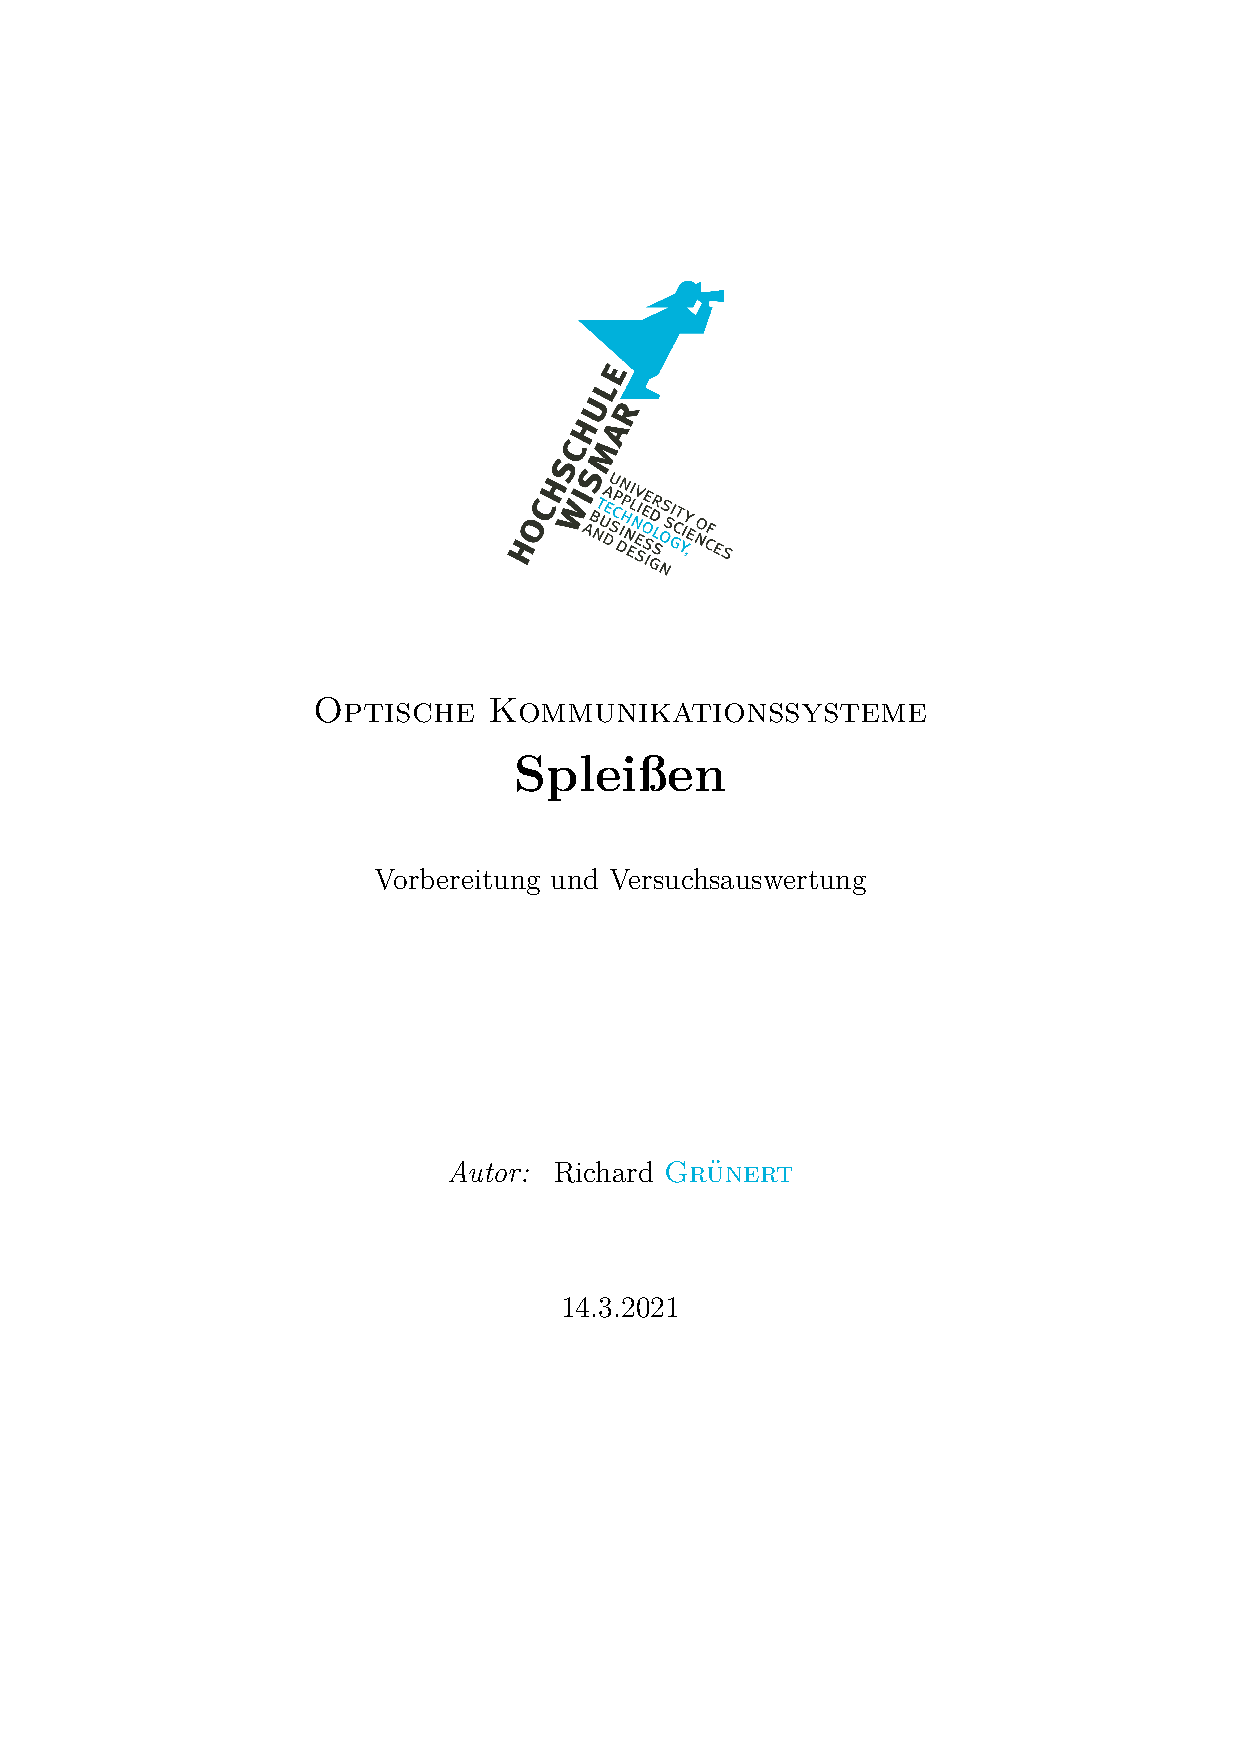
\includepdf{./titlepage/titlepage.pdf}
  \clearpage
  \setcounter{page}{1}
%%%%%%%%%%%%%%%%%%%%%%%%%%%%%%%%%%%%%

\section{Vorbereitungsaufgaben}

\subsection{}
Die Grundfrequenz der dargestellten (periodischen) Datenfolge ist

$$f = \frac{1}{T} = \frac{1}{1 \, \si{\micro\second}} = 1 \, \si{\mega\hertz}$$

\subsection{}

\begin{figure}[H]
\begin{center}
  \begin{circuitikz}
    \draw (0,0) to[R, l=$R$, o-] (2,0) to[L, l=$L$] (4,0) -- (7,0) to[short, -o]
    (9,0);
    \draw (5,0) to[R, l=$G$, *-*] (5,-3);
    \draw (7,0) to[C, l=$C$, *-*] (7,-3);
    \draw (0,-3) to[short, o-o] (9,-3);
  \end{circuitikz}
\end{center}

\caption{Ersatzschaltbild einer Kupferdoppelader}
\end{figure}

Die Kupferdoppelader kann im Ersatzschaltbild durch einen Widerstand $R$, eine
Induktivität $L$, einem Leitwert $G$ und eine Kapazität $C$
modelliert werden, welche alle proportional zur Länge der Leitung sind. Die auf
die Leitungslänge bezogenen
Parameter des Ersatzschaltbildes werden in der Leitungstheorie auch
\emph{Leitungsbeläge} genannt. \\ Der Widerstand $R$ der Leitung entsteht durch den spezifischen
Widerstand des Materials $\rho$, der Querschnittsfläche $A$ und der Länge $l$ der Leitung
nach $$R = \rho \cdot \frac{l}{A}, $$ wobei zu beachten ist, dass 
die gesamte Leitungslänge, also beide Adern bei der Doppelader, als Länge in die
Berechnung eingeht. Zudem ist der Widerstandsbelag frequenzabhägig (Skineffekt).

Da die gesamte Doppelader eine Spule mit nur einer Windung darstellt, tritt eine
Induktivität $L$ auf. 
$$ L = (N^2) \cdot \mu \cdot \frac{A}{l} $$
Praktisch wird weiterhin zwischen einer äußeren Induktivität (magnet.
Eigenschaften, Geometrie des
Leiters) und einer inneren Induktivität (Wechselfelder innerhalb des Leiters, Skineffekt) unterschieden

Die Kapazität $C$ entsteht durch die Kondensatorwirkung der zwei dicht
beeinanderliegenden Adern.
$$ C = \epsilon \cdot \frac{A}{d}$$

Die dielektrischen Verluste zwischen beiden Adern werden durch den Leitwert $G$
(Ableitungsbelag) gekennzeichnet, welcher auch über den Verlustwinkel $\delta$
der Kapazität des Dielektrikums bestimmt ist.

Durch frequenzabhägige Elemente ($L$, $C$) im Ersatzschaltbild wird die
Übertragungsfunktion der Doppelader ebenfalls frequenzabhägig und weicht damit
von einer idealen, frequenzunabhägigen Leitung ab. Aus dem
Ersatzschaltbild lässt sich das Tiefpassverhalten der Doppelader herleiten.
Außerdem können durch Bildung eines Schwingkreises unerwünschte Resonanzerscheinungen auftreten.

\subsection{}

\begin{figure}[H]
	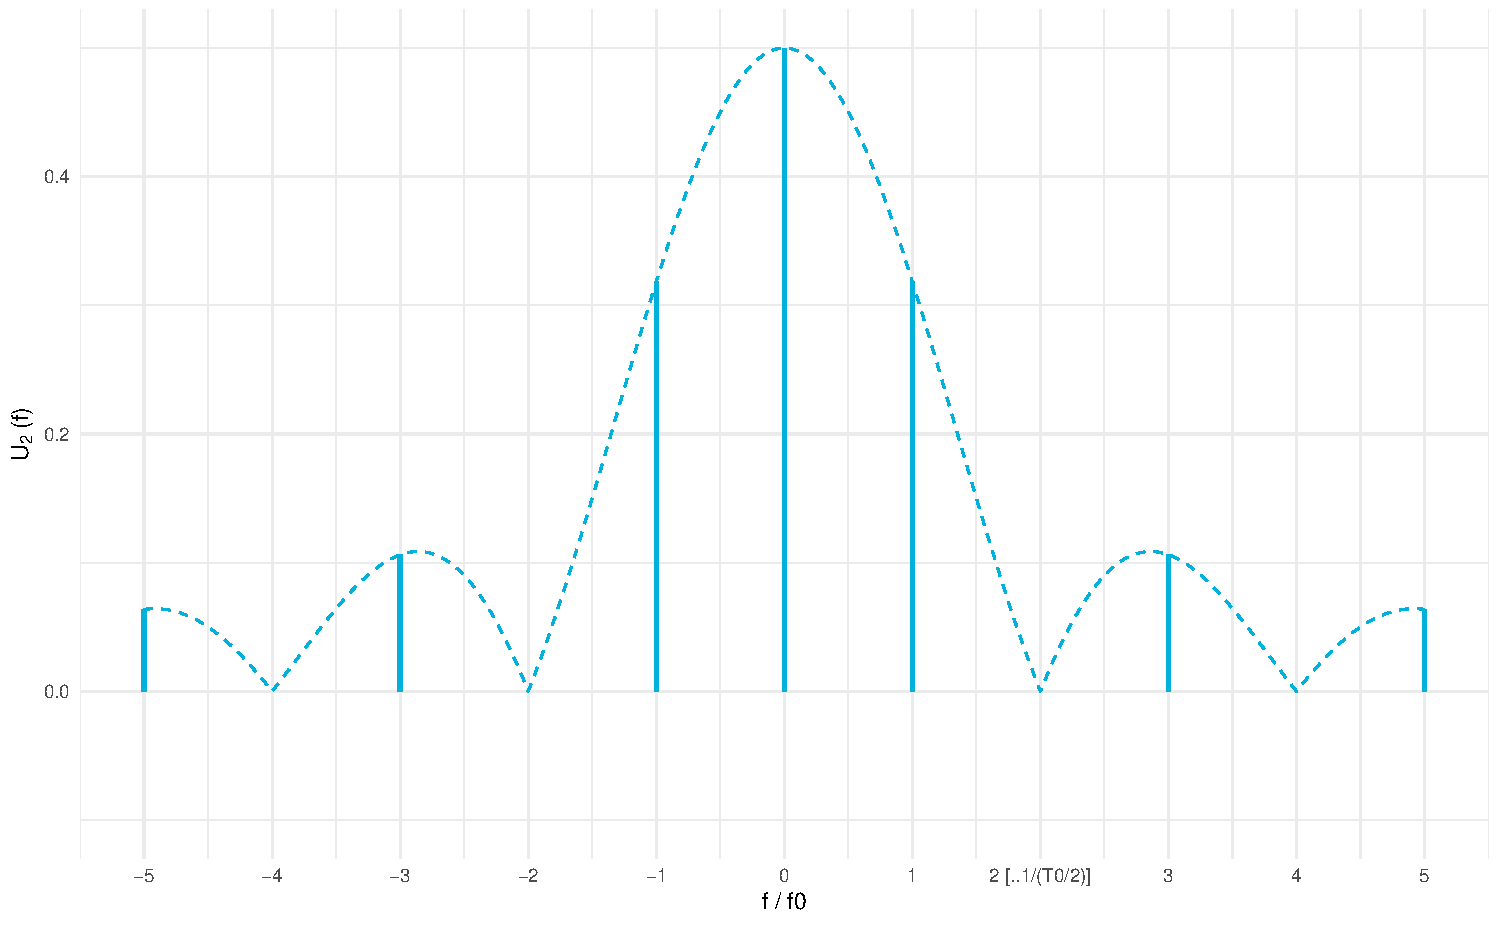
\includegraphics[width=\textwidth]{1_3/Si}
  \caption{Teil des Spektrums der periodischen 1010-Folge mit der Si-Funktion als Einhüllende}
\end{figure}

\begin{figure}[H]
	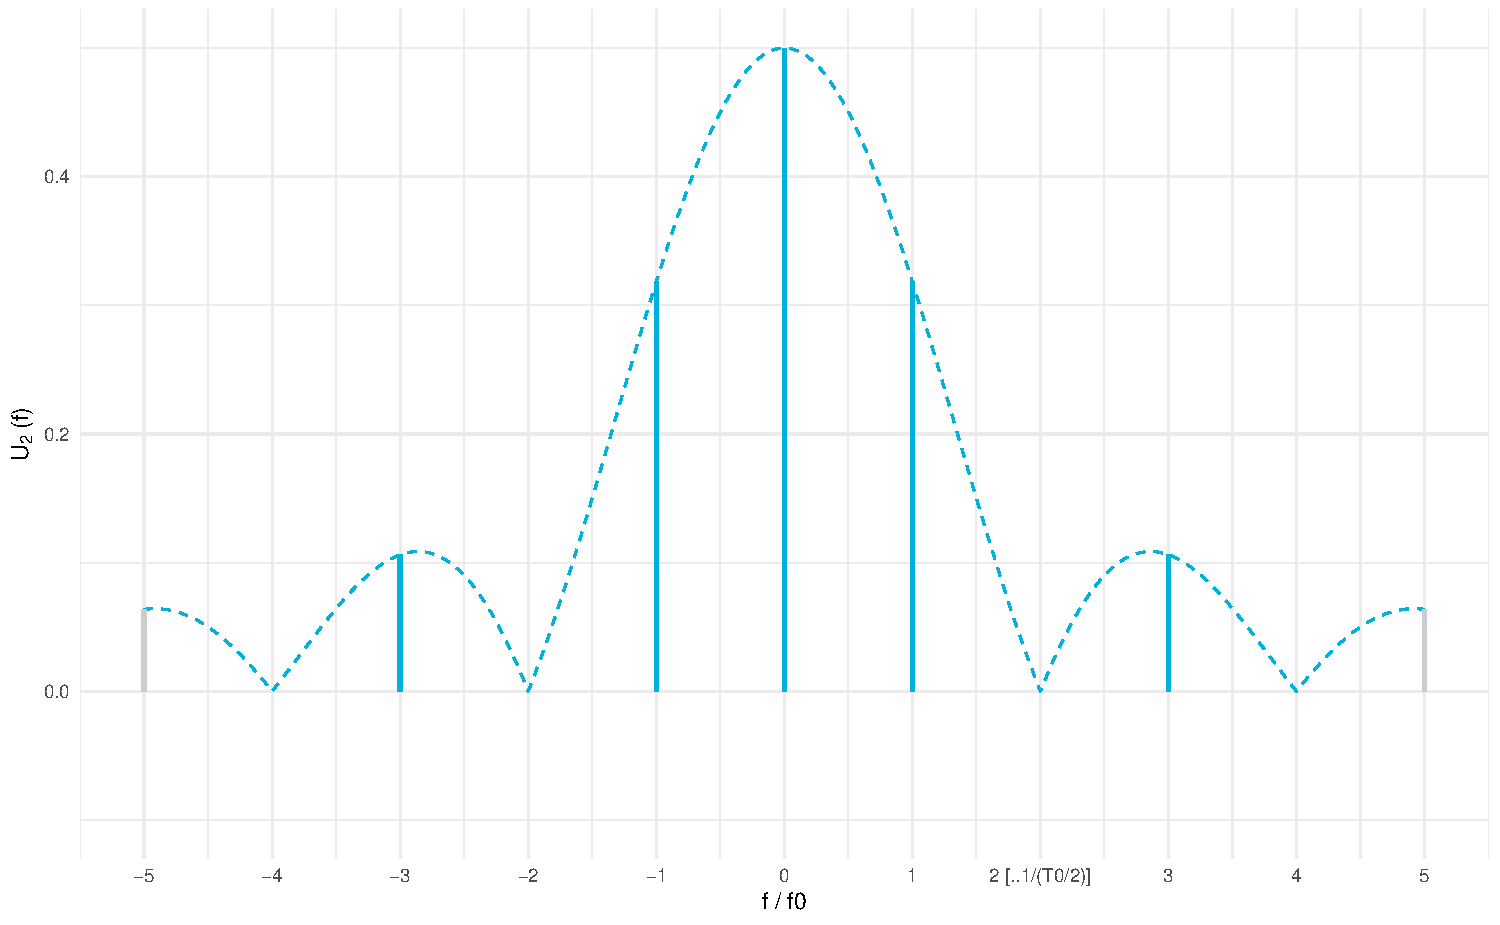
\includegraphics[width=\textwidth]{1_3/Si_filtered}
  \caption{Beispielhaftes Spektrum der periodischen 1010-Folge mit TP-Filtercharakteristik der
    Doppelader}
\end{figure}


Da hier eine periodische Folge gewählt wurde, entsteht ein diskretes
Amplitudenspektrum, welches durch Fouriersynthese wieder in die Ursprungsfolge
umgewandelt werden kann. Fehlen nun einige Spektrallinien  durch die
Tiefpasscharakteristik der Doppelader (in Abb. 3 grau gekennzeichnet), weicht die Folge nach
der Synthese von der Originalfolge ab (Abb. 4).

\begin{figure}[H]
	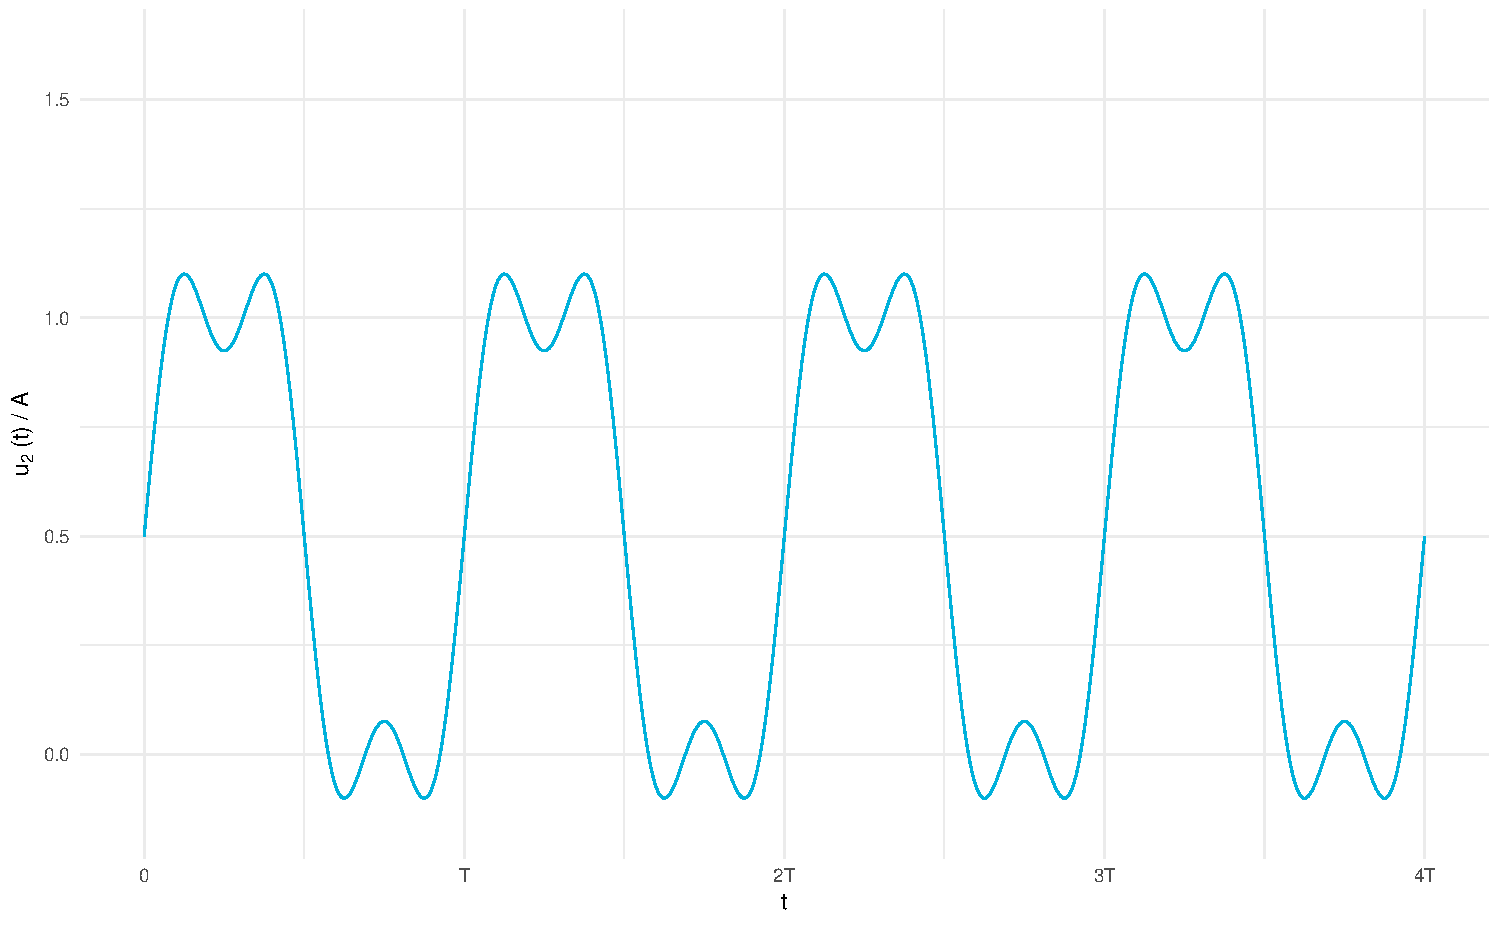
\includegraphics[width=\textwidth]{1_3/loss}
  \caption{ Auswirkung des spektralen Verlusts im Zeitbereich }
\end{figure}


\subsection{}

Wie in Abb. 4 zu sehen, ist die empfangene Rechteckfolge uneindeutiger als die
Gesendete. Die Wahrscheinlichkeit für eine Fehlinterpretation eines Bits ist
daher höher, wodurch fehlerhafte Datenübertragungen zustande kommen können.

\subsection{}

Die Grundfrequenz der 1010-Folge ist die Hälfte der Übertragungsrate von $f_1 = 704 \,
\textrm{kbit/s}$, da in einer Grundperiode der 1010-Folge
bei dieser Datenrate theoretisch 2 bits übertragen werden könnten.



Das auf die Grundfrequenz normierte Amplitudenspektrum ergibt sich mit dem
Tastverhältnis von $D = 0.5$ zu
$$\mid \underline{X}_n \mid = A \cdot \frac{1}{2} \cdot \textrm{Si}(n \pi \cdot \frac{1}{2}) $$



Die periodische 1010-Folge ist zur Messung gut geeignet, da es durch die höchstmögliche Frequenz einer Bitfolge das worst-case-Szenario darstellt.

\subsection{}

Wobbeln ist eine Methode der Frequenzanalyse eines Systems und beschreibt das
Durchlaufen eines bestimmten Frequenzbereiches mit Sinus-Funktionen. 

\subsection{}

a) Der Netzwerkanalysator misst selbstständig mit einer hohen Auflösung durch
Wobbeln der Kupferdoppelader. Die Übertragungsfunktion wird danach automatisch dargestellt.

\noindent b) Zur Messung der Übertragungsfunktion wurde die $704 \,
\textrm{kbit}/\textrm{s}$-Folge gewählt, da der Abstand der Spektrallinien gegenüber der $2
\, \textrm{Mbit}/\textrm{s}$-Folge geringer ist, was eine höhere Auflösung der
Messwerte erlaubt.

Die Messung erfolgte durch Senden einer periodischen 1010-Rechteckfolge mit konstanter Amplitude
durch die Kupferdoppelader. Durch die FFT-Analyse am Oszilloskop wurde das
gemessene, ausgangsseitige Spektrum mit dem eingangsseitigen Spektrum
verglichen. Die Differenzen der Amplituden zu den jeweiligen Frequenzen (in
$\si{\deci\bel}$) stellen die Übertragungsfunktion der Doppelader dar.

\section{Versuchsaufgaben}

\subsection{}

\begin{figure}[H]
	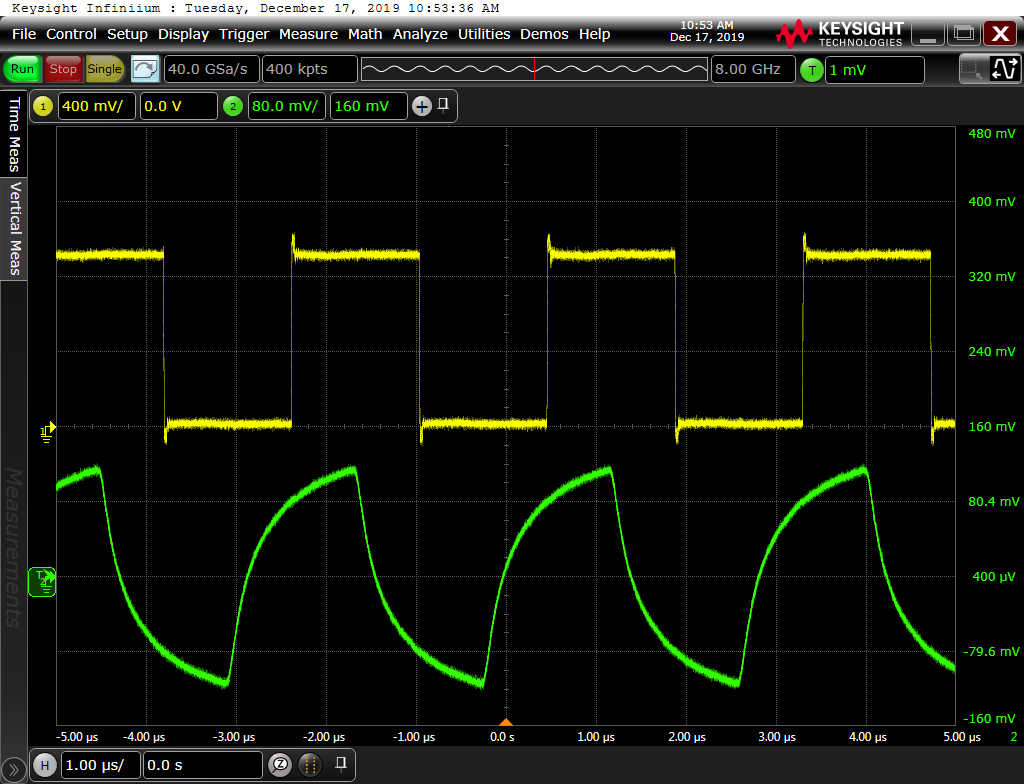
\includegraphics[width=\textwidth]{Versuch/704kbit Zeitbereich}
  \caption{Darstellung der 704 kbit/s -Folge im Zeitbereich, gelb:
    Eingangsseitig, grün: Ausgangsseitig}
\end{figure}

Aus dem Bild der Signale im Zeitbereich (Abb. 5) lassen sich die
Phasenverschiebung und Amplitudenänderung des Ausgangssignals erkennen. Das
Ausgangssignal ist durch die vorherige Umformung (Converter) symmetrisch um 0V (kein Gleichanteil) und
hat die selbe Frequenz wie das Eingangssignal. Außerdem kann man den Lade-und
Entladeeinfluss der Doppeladerkapazität erkennen.

\begin{figure}[H]
	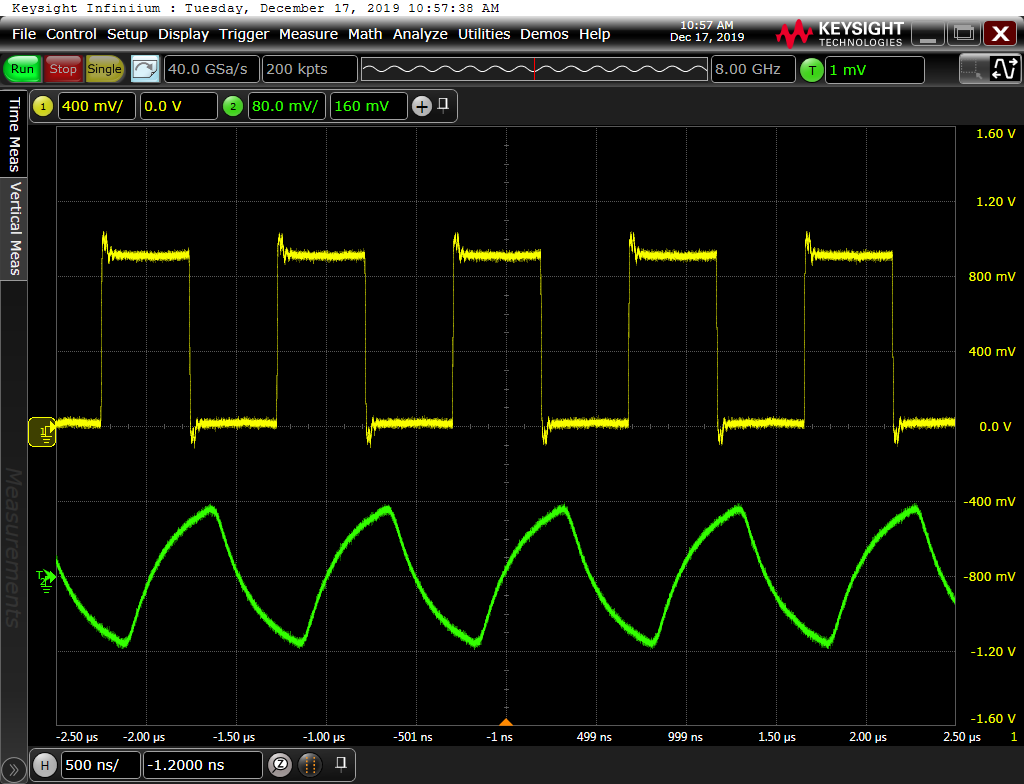
\includegraphics[width=\textwidth]{Versuch/2Mbit 1010 Zeitbereich}
  \caption{Darstellung der 2 Mbit/s -Folge im Zeitbereich, gelb:
    Eingangsseitig, grün: Ausgangsseitig}
\end{figure}

In Abb. 6 wurde die Datenübertragungsrate auf $2 \, \textrm{Mbit/s}$ erhöht. Man
erkennt die stärkere Amplitudenverringerung des Ausgangssignals bei der höheren Frequenz. 

\pagebreak 
\noindent b) Zur Ermittlung der Übertragungsfunktion der Doppelader wurde dann die
FFT-Funktion des Oszilloskops verwendet.

\begin{figure}[H]
	\includegraphics[width=\textwidth]{Versuch/704kbit FFT mit Peaks}
  \caption{FFT des Eingangs- und Ausgangssignals mit den Amplitudenwerten}
\end{figure}

\begin{figure}[H]
	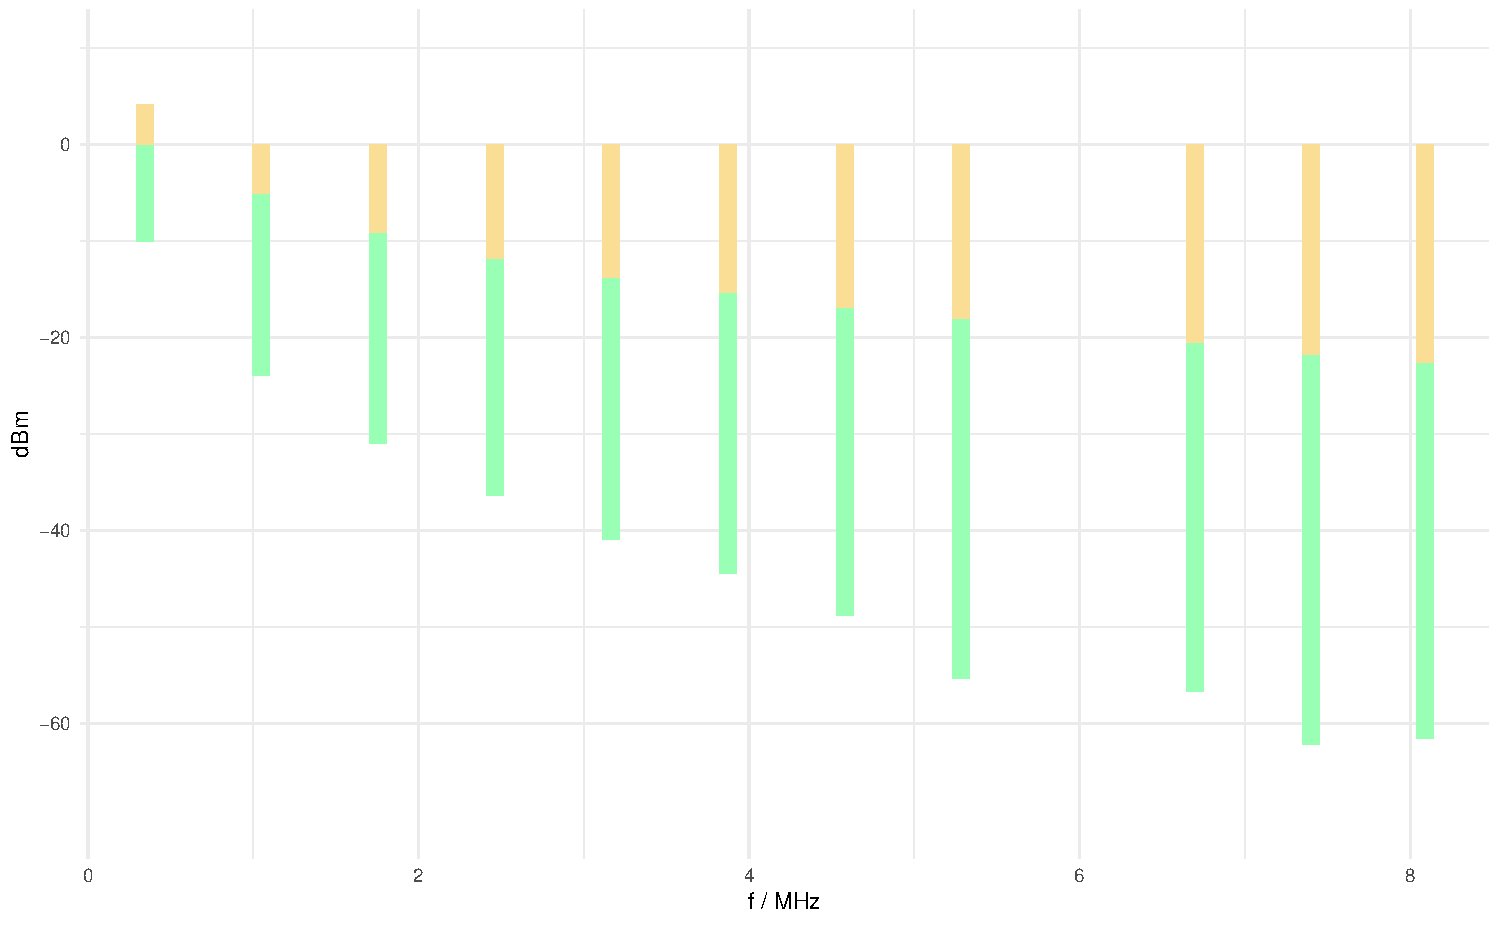
\includegraphics[width=\textwidth]{2_1/2_1_704kbit_Amplivergleich}
  \caption{Amplitudenvergleich des Eingangs (gelb)- und Ausgangssignals (grün)
    über der Frequenz}
\end{figure}

\begin{figure}[H]
	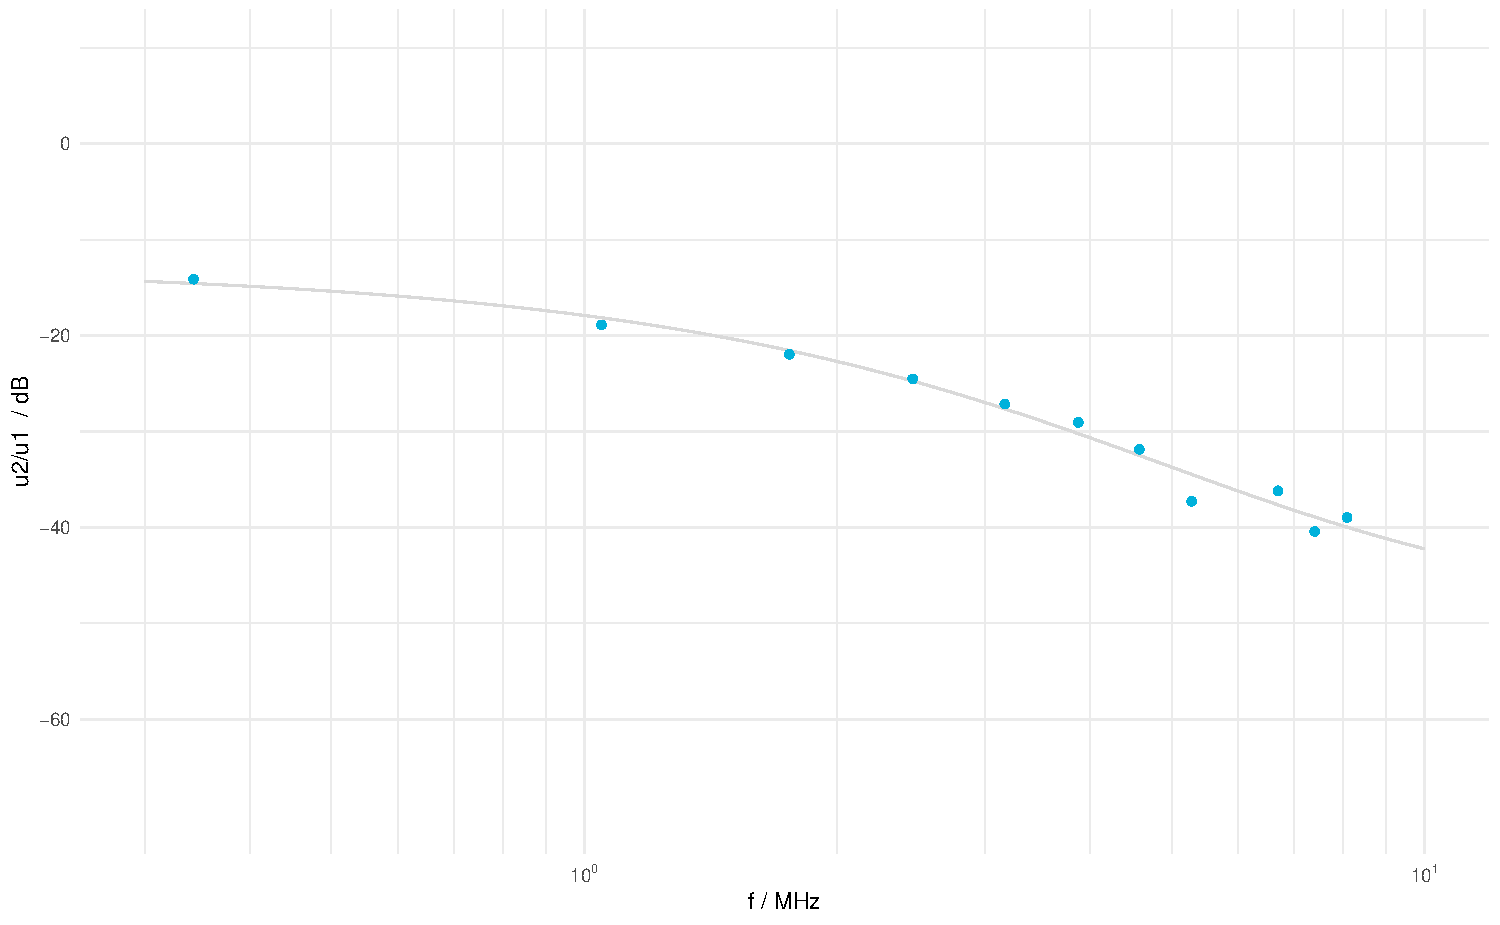
\includegraphics[width=\textwidth]{2_1/2_1_704kbit_Übertragungsfunktion}
  \caption{Übertragungsfunktion aus den Amplitudendifferenzen}
\end{figure}

In Abb. 8 sind die aus der FFT erhaltenen Amplitudenwerte von Ein- und
Ausgangssignal zum Vergleich dargestellt.

Die Übertragungsfunktion
$$ G(f) = \frac{U_2(f)}{U_1(f)} $$

kann durch die Amplitudenmesswerte im logarithmischen Maß als Differenz
$$G(f) = \textrm{dBm}_{\textrm{Ausgang}}-\textrm{dBm}_{\textrm{Eingang}}$$

\noindent dargestellt werden, wie in Abb. 9 zu sehen.
Man erkennt die steigende Dämpfung mit der Frequenz, also typisches
Tiefpassverhalten.

\subsection{}


\begin{figure}[H]
	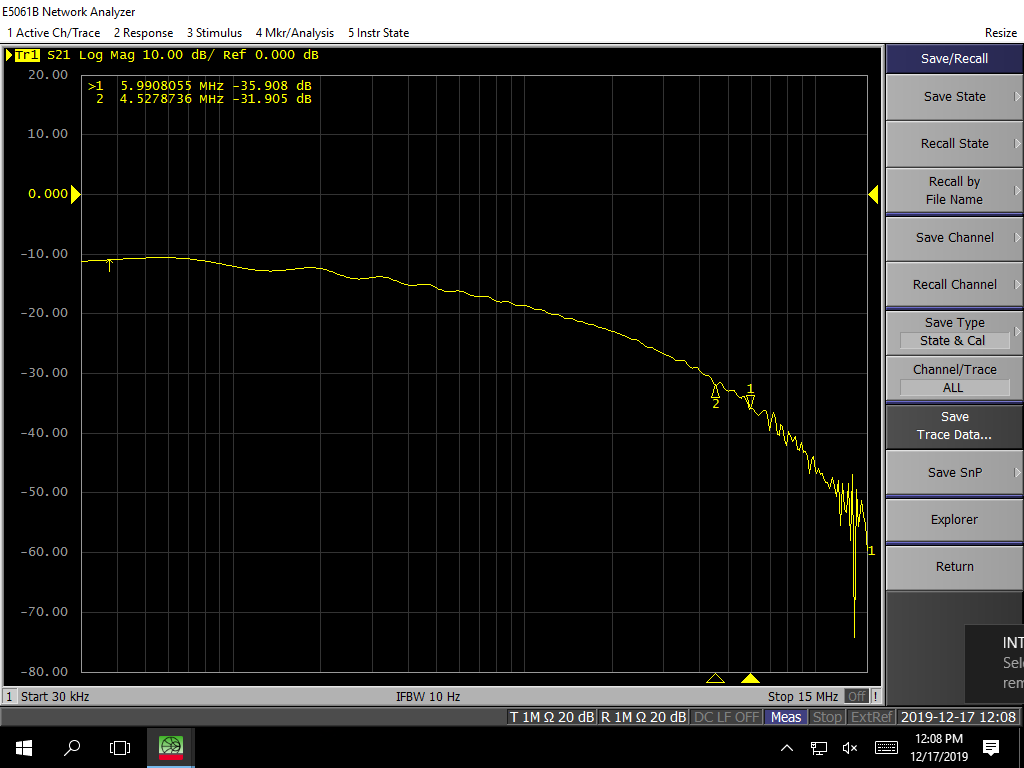
\includegraphics[width=\textwidth]{Versuch/nwa wobbel 30khz 15mhz}
  \caption{Mit dem NWA aufgenommene Übertragungsfunktion}
\end{figure}

Mit dem Netzwerkanalysator konnte die Übertragungsfunktion der Doppelader
automatisch ermittelt werden. Das Frequenzintervall wurde von $30 \,
\si{\kilo\hertz}$ bis $15 \, \si{\mega\hertz}$ eingestellt. 

Aus den Abbildungen 9 und 10 lässt sich die Übereinstimmung der durch die beiden
Messmethoden ermittelten Übertragungsfunktionen feststellen (Bsp: Wert bei 5MHz in beiden ca. -20dB).

\end{document}
